\documentclass{article}

\usepackage{amsmath}
\usepackage{graphicx}

\title{Report 6: Convolutional Neural Network}
\author{Hoai Nam Le}

\begin{document}

\maketitle

\section{Network Architecture}

A convolutional neural network (CNN) was
implemented from scratch using NumPy and OpenCV.

The network architecture contains:

\begin{itemize}
    \item Convolution layer
    \item ReLU activation
    \item Max pooling layer
    \item Fully connected layer
    \item Softmax output layer
\end{itemize}

Architecture:

\begin{verbatim}
Input 28x28 -> Convolution 3x3 -> ReLU -> MaxPooling 2x2 -> Flatten 
-> Fully Connected -> Softmax
\end{verbatim}

The convolution layer extracts image features
using a learnable kernel.

\[
output(i,j)=\sum region \times kernel
\]

The ReLU activation introduces non-linearity:

\[
ReLU(x)=max(0,x)
\]

Max pooling reduces the spatial size while
keeping important features.

The fully connected layer performs classification.

Softmax converts outputs into probabilities:

\[
Softmax(x_i)=
\frac{e^{x_i}}
{\sum_j e^{x_j}}
\]

\section{Training Pipeline}

The CNN training pipeline is:

\begin{verbatim}
Image -> Convolution -> ReLU -> Pooling -> Flatten -> Fully Connected Softmax 
-> Cross Entropy Loss -> Backpropagation -> Gradient Descent
\end{verbatim}

The model was trained using gradient descent.

Weights were updated using:

\[
W = W - r \nabla W
\]

where:
\begin{itemize}
    \item $W$ is the weight matrix
    \item $r$ is the learning rate
    \item $\nabla W$ is the gradient
\end{itemize}

Cross entropy loss was used:

\[
Loss = -\log(p_y)
\]

\section{Dataset}

The MNIST handwritten digit dataset was used.

The dataset contains 10 classes:

\[
0,1,2,\dots,9
\]

Each image has size:

\[
28 \times 28
\]

\section{Evaluation Metrics}

The network was evaluated using classification
metrics.

Accuracy measures the percentage of correct
predictions.

\[
Accuracy=
\frac{Correct Predictions}
{Total Predictions}
\]

Experimental result:

\begin{verbatim}
Accuracy = 0.84
\end{verbatim}

\section{Discussion}

The CNN architecture successfully implemented:

\begin{itemize}
    \item Convolution
    \item Pooling
    \item Softmax classification
    \item Backpropagation
    \item Gradient descent
\end{itemize}

The loss decreased during training, showing that
the model learned from the dataset.

The accuracy is still limited because:
\begin{itemize}
    \item Only one convolution kernel was used
    \item Only the fully connected layer was trained
    \item The network architecture is simplified
\end{itemize}

\section{Training Result Figure}

\begin{figure}[h]
    \centering
    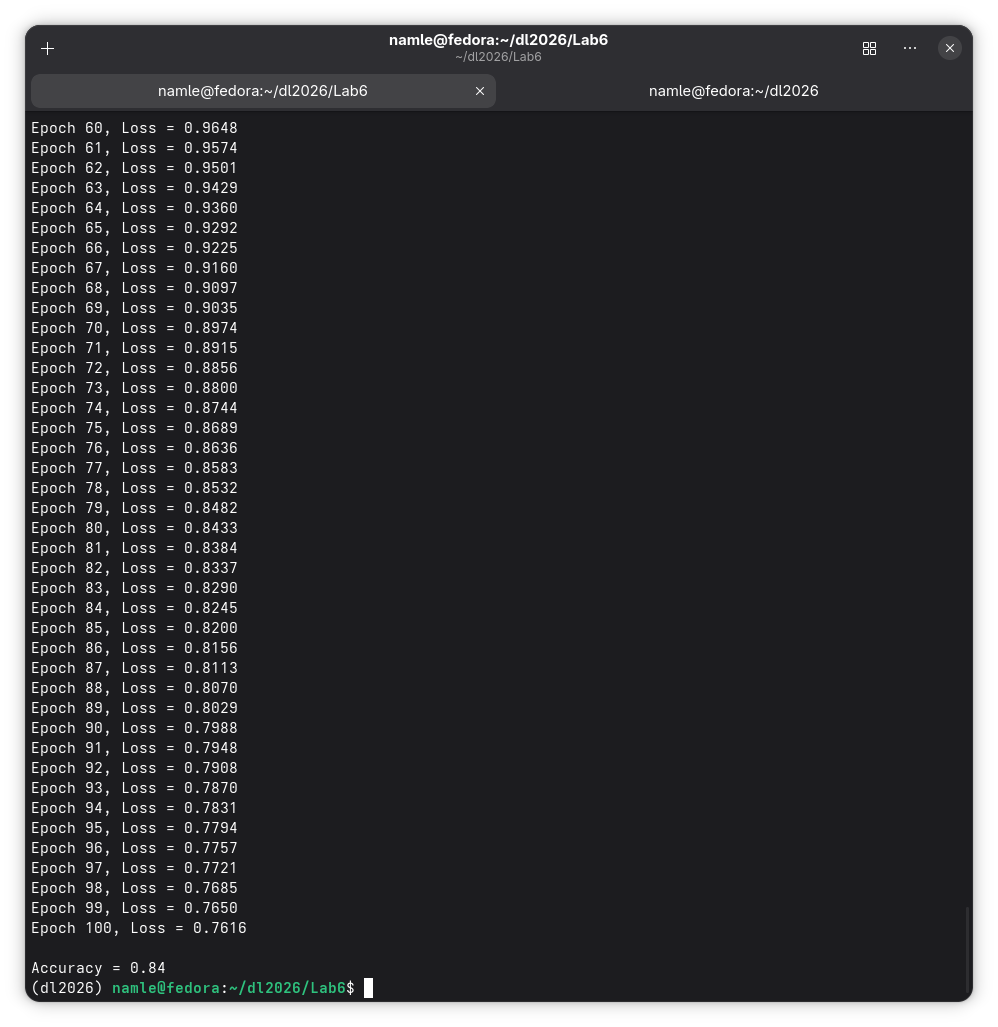
\includegraphics[width=0.9\linewidth]{cnn_results.png}
    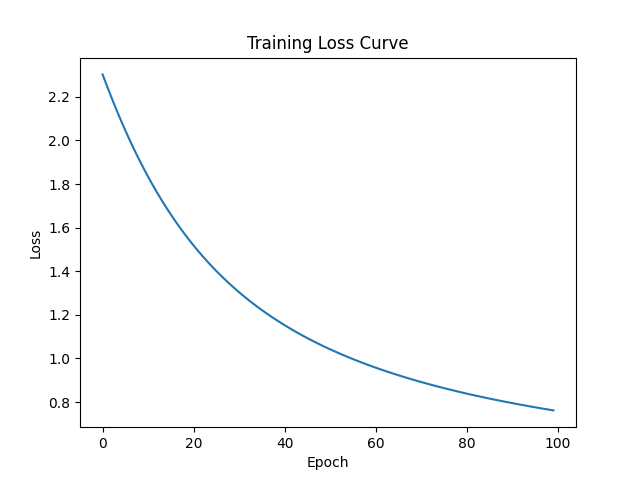
\includegraphics[width=0.9\linewidth]{loss_curve.png}
    \caption{CNN training result and accuracy}
\end{figure}

\end{document}